%Preamble
\documentclass[12pt,a4paper]{article}
\usepackage[top=20mm, bottom=20mm, left=20mm, right=20mm]{geometry}
\usepackage[utf8]{inputenc}
\usepackage{fancyhdr} \setlength{\headheight}{15pt}
\usepackage{lastpage}
\usepackage[magyar]{babel}
\usepackage{amsmath}
\usepackage{amsthm}
\usepackage{empheq}
\usepackage{enumitem}
\usepackage{float}
\usepackage{verbatim}
\usepackage{hyperref}
\usepackage{multicol}
\usepackage{blkarray}
\usepackage[most]{tcolorbox}
\usepackage{tikz}
\usepackage{pgfplots}
\usepackage{picture}
\usepackage{graphicx}
\usepackage{makecell}
\usepackage{eso-pic}
\usepackage[executable=python3.10.exe]{pyluatex}

\pagestyle{fancy}
\pgfplotsset{compat=1.18}
\setlength{\headheight}{15.21004pt}

\def\mx#1{\mathbf{#1}}
\def\vec#1{\underline{\mathbf{#1}}}
\def\m{\; \left[\mathrm{m}\right]}
\def\mili{\; \left[\mathrm{mm}\right]}
\def\mm{\; \left[\mathrm{m^2}\right]}
\def\mmmm{\; \left[\mathrm{m^4}\right]}
\def\i{\left(i\right)}
\def\ui#1{\left(#1\right)}
\def\SI{\; \left[\mathrm{SI}\right]}
\def\Nm{\; \left[\mathrm{Nm}\right]}
\def\N{\; \left[\mathrm{N}\right]}
\def\kN{\; \left[\mathrm{kN}\right]}
\def\futyi{\cdot 10^{9}}
\def\fos{\; \left[-\right]}
\def\Gpa{\; \left[\mathrm{GPa}\right]}
\def\rads{\; \left[\mathrm{\frac{rad}{s}}\right]}
\def\Hz{\; \left[\mathrm{Hz}\right]}
\def\kg{\; \left[\mathrm{kg}\right]}
\def\kgpm{\; \left[\mathrm{\frac{kg}{\; m^3}}\right]}

\lhead{BMEGEMMBXVE, VEM alapjai 2.HF}
\cfoot{\thepage\ / \pageref{LastPage}}
\rhead{Németh Áron Imre, D1J5ZG}

\begin{python}
    import sympy as sp
    from sympy.printing.latex import LatexPrinter, print_latex
    from sympy import latex
    from calc.vem_hf2_calc import calculate
    from calc.var_print import printer, print_matrix, prin_TeX, my_latex

    V=calculate(2,2,2)
\end{python}

\begin{document}

\AddToShipoutPictureFG*{
    \put(12cm,27.33cm){
        \makebox(3.85cm, -1.35cm){
            \hfill Németh Áron Imre
        }
    }
    \put(12cm,26.67cm){
        \makebox(3.2cm,-1.2cm){
            \hfill D1J5ZG
        }
    }
    \put(15.45cm,26cm){
        \makebox(-3.6cm,-1cm){
            \hfill 
\includegraphics[height=6mm]{./static/signature.pdf} \hfill
        }
    }

    \put(9.5cm,25cm){
        \makebox(3.5mm,-1.5cm){1}
        \makebox(20mm,-1.5cm){2}
        \makebox(2.5mm,-1.5cm){2}
        \makebox(20mm,-1.5cm){2}
    }
    \put(4.35cm, 5.725cm){
        \makebox(0mm,0mm){{$\pyc{prin_TeX(V["f_1_a"],3)}$}}
        \makebox(47mm,0mm){{$\pyc{prin_TeX(V["f_2_a"],3)}$}}
        \makebox(0mm,0mm){{$\pyc{prin_TeX(V["f_3_a"],3)}$}}
        \makebox(48mm,0mm){{$\pyc{prin_TeX(V["f_1_b"],3)}$}}
        \makebox(0mm,0mm){{$\pyc{prin_TeX(V["f_2_b"],3)}$}}
        \makebox(47mm,0mm){{$\pyc{prin_TeX(V["f_3_b"],3)}$}}
    }
    \put(4.35cm, 4.5cm){
        \makebox(0mm,0mm){{$\pyc{prin_TeX(V["f_1_c"],3)}$}}
        \makebox(47mm,0mm){{$\pyc{prin_TeX(V["f_2_c"],3)}$}}
        \makebox(0mm,0mm){{$\pyc{prin_TeX(V["f_3_c"],3)}$}}
        \makebox(48mm,0mm){{$\pyc{prin_TeX(V["f_1_d"],3)}$}}
        \makebox(0mm,0mm){{$\pyc{prin_TeX(V["f_2_d"],3)}$}}
        \makebox(47mm,0mm){{$\pyc{prin_TeX(V["f_3_d"],3)}$}}
    }
}
\begin{figure}[H]
    \centering
    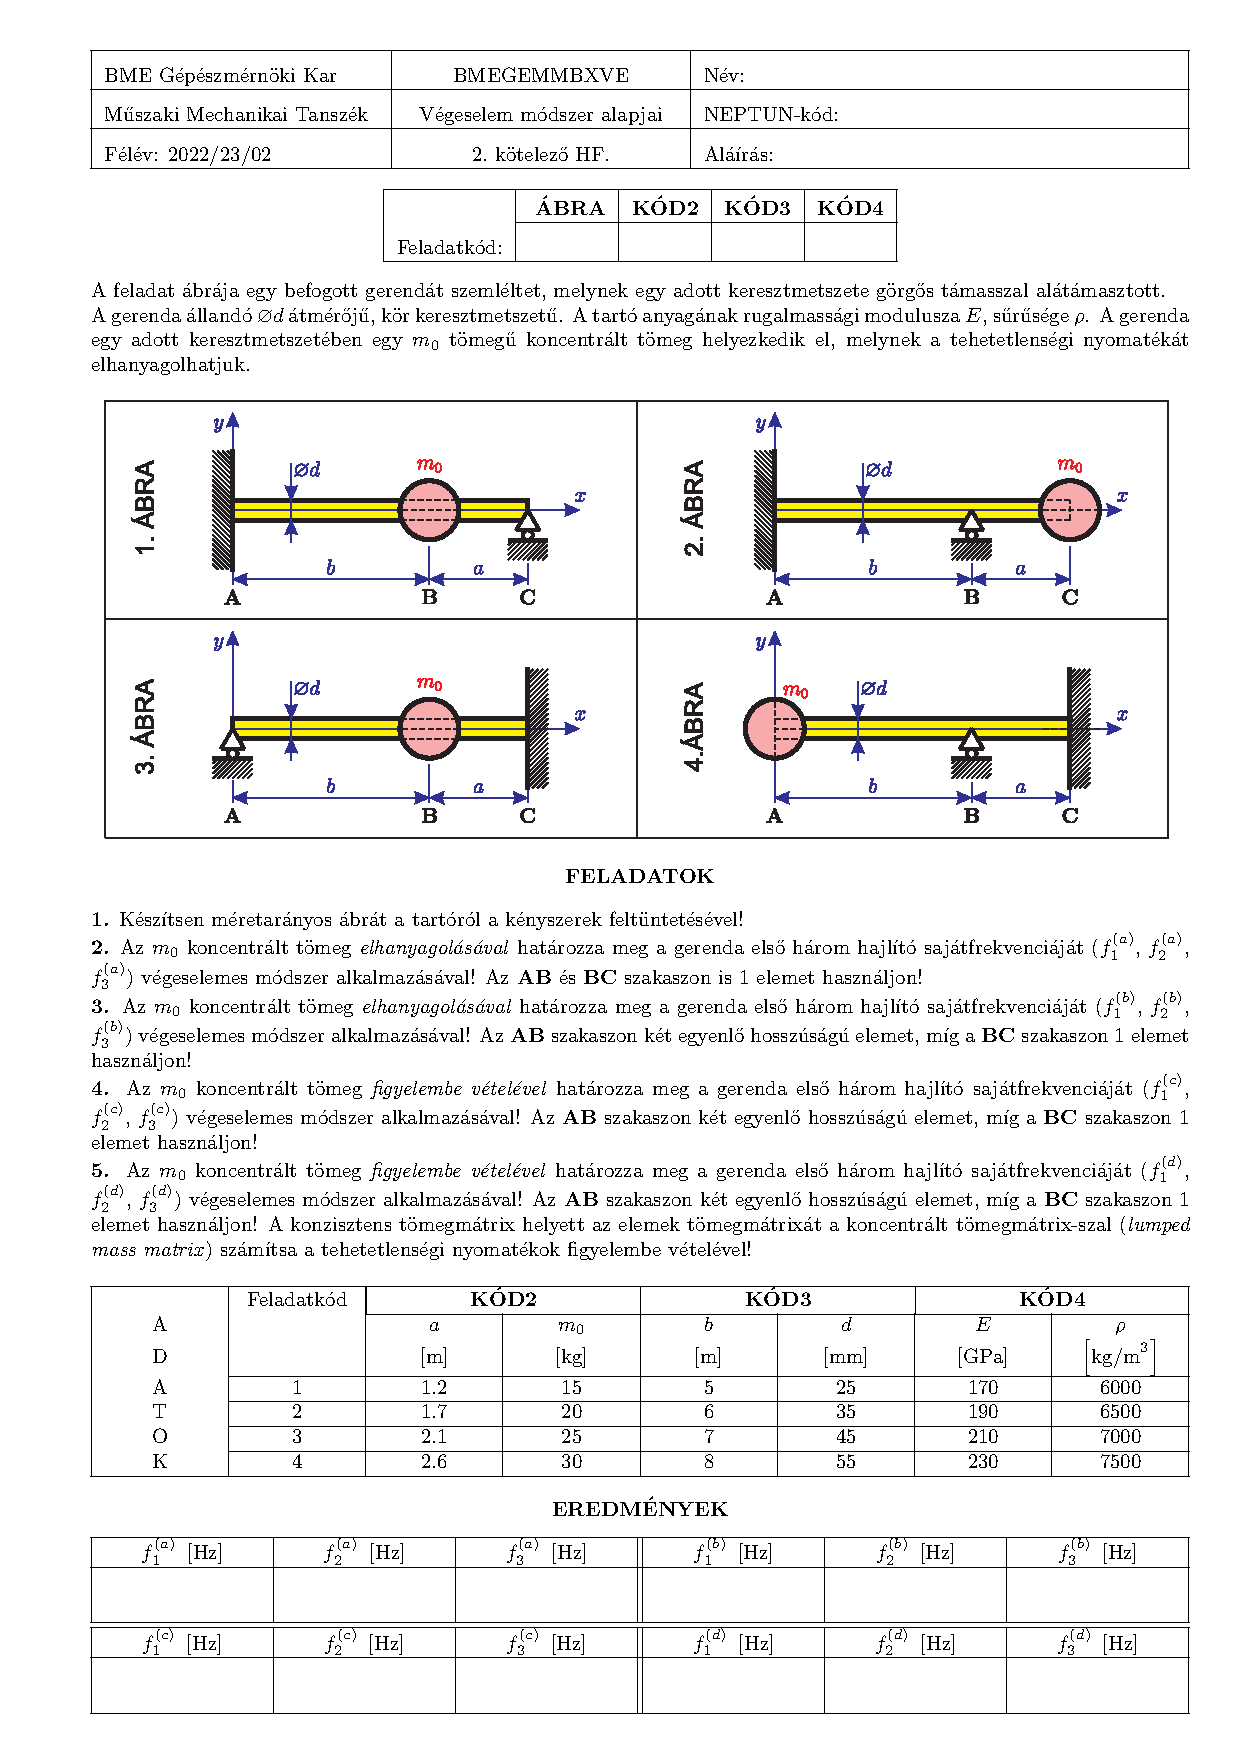
\includegraphics[
        %pages=1,
        width=\linewidth,
        %pagecommand=\thispagestyle{fancy}
    ]
    {static/vem_hf2_titlepage.pdf}
\end{figure}



\section{A szerkezet méretarányos ábrájának elkészítése}
\subsubsection*{Adatok:}

\begin{multicols}{2}
    \begin{itemize}
        \item $a=\pyc{prin_TeX(V["a"],1)}\m$
        \item $b=\pyc{prin_TeX(V["b"])}\m$
        \item $d=\pyc{prin_TeX(V["d_mm"])}\mili$
    \end{itemize}
    \columnbreak
    \begin{itemize}
        \item $E=\pyc{prin_TeX(V["E_GPa"])} \Gpa$
        \item $m_0=\pyc{prin_TeX(V["m_0"])} \kg$
        \item $\rho=\pyc{prin_TeX(V["rho"])} \kgpm $
    \end{itemize}
\end{multicols}

\subsection{A szerkezet léptékhelyes ábrája}
A szerkezet méretarányos ábrája esetünkben az alábbi módon néz ki:

\subsection{A szerkezet végeselem modelljének ábrája}
Az alábbi ábrán látható a szerkezet VEM modellje:

\section{Két BEAM elem használata}
A VEM modell két \textbf{BEAM} elemből áll, egyik elem az \textbf{AB} szakaszon,
míg a második elem a \textbf{BC} szakaszon helyezkedik el. A számítások során
a koncentrált tömeget \textit{elhanyagoljuk}, valamint \textit{konzisztens} tömegmátrixot
használunk.
\subsection{Csomópontok, elemek definiálása}
\subsubsection{Csomópontok definiálása}
Az alábbi táblázatban láthatóak a különböző csomópontok $x$ illetve
$y$ koordinátái:
\begin{center}
    \begin{tabular}{|c|c|c|}
        \hline
        Csomópont & x koordináta & y koordináta \\
        \hline
        \hline
        1         & 0            & $0$          \\
        \hline
        2         & $b$          & $0$          \\
        \hline
        3         & $a+b$        & $0$          \\
        \hline
    \end{tabular}
\end{center}

\subsubsection{Elemek hozzárendelése a csomó pontokhoz}
Az alábbi táblázat tartalmazza a csomópont-elem hozzárendeléseket:
\begin{center}
    \begin{tabular}{|c|c|c|}
        \hline
        Elemszám & Lokális 1. csomópont & Lokális 2. csomópont \\
        \hline
        \hline
        1        & 1                    & 2                    \\
        \hline
        2        & 2                    & 3                    \\
        \hline
    \end{tabular}
\end{center}

\subsection{Elemek tulajdonságainak meghatározása}
\subsubsection{Az elemek hosszainak meghatározása}
A rúdak hosszait az alábbi általános képlet segítségével tudjuk
könnyen kiszámítani:
\begin{tcolorbox}[ams equation]\label{eq:L_i}
    L^{\left(i\right)}=\sqrt{\left(x^{\left(i\right)}_2-x^{\left(i\right)}_1\right)^2+
        \left(y^{\left(i\right)}_2-y^{\left(i\right)}_1\right)^2}
\end{tcolorbox}
\noindent Ezen képletet alkalmazva a rúdak hosszai numerikusan az alábbiak:
\begin{multicols}{2}
    \begin{itemize}
        \item $L_1^{\ui{a}}=\pyc{prin_TeX(V["L_1_a"])} \m$
    \end{itemize}
    \columnbreak
    \begin{itemize}
        \item $L_2^{\ui{a}}=\pyc{prin_TeX(V["L_2_a"])} \m$
    \end{itemize}
\end{multicols}

\subsubsection{Az elemek keresztmetszeteinek tulajdonságainak meghatározása}
Mivel mindegyik elemünk kör keresztmetszetű, így az alábbi összefüggésekkel számíthatjuk ki a keresztmetszetek területét
és másodrendű nyomatékait:
\begin{tcolorbox}[ams equation]
    A^{\i}=\frac{\left(d^{\i}\right)^2  \pi}{4} \hspace{40mm}
    I_z^{\i}=\frac{\left(d^{\i}\right)^4  \pi}{64}
\end{tcolorbox}
\noindent Mivel az elemk keresztmetszeteinek átmérője azonos,
ezért az elemek keresztmetszeteinek területei valamint másodrendű nyomatékai
megegyeznek. Tehát a keresztmetszetek területei és másodrendű nyomatékai numerikusan:
\begin{multicols}{2}
    \begin{itemize}
        \item $A_1^{\ui{a}}=A_2^{\ui{a}}=\pyc{prin_TeX(V["A"]*10**4,3)} \cdot 10^{-4}\mm$
    \end{itemize}
    \columnbreak
    \begin{itemize}
        \item ${I_z}_1^{\ui{a}}={I_z}_2^{\ui{a}}=\pyc{prin_TeX(V["Iz"]*10**8,3)} \cdot 10^{-8} \mmmm$
    \end{itemize}
\end{multicols}
\subsection{Az elemi merevségi mátrixok meghatározása}
Most hogy már ismerjük a keresztmetszetek területét, másodrendű nyomatékait valamint rugalmassági modulusait, az alábbi
\textbf{BEAM} gerendaelemre vonatkozó összefüggéssel meghatározhatjuk a különböző elemek merevségi mátrixait:
\begin{tcolorbox}[ams equation]\label{eq:K_i}
    \mx{K}^{\i}=\frac{{I_z}_i E_i}{{L_i}^3}
    \begin{bmatrix}
        12    & 6 L_i        & -12    & 6 L_i        \\
        6 L_i & \; 4 {L_i}^2 & -6 L_i & \; 2 {L_i}^2 \\
        -12   & -6 L_i       & \; 12  & -6 L_i       \\
        6 L_i & \; 2 {L_i}^2 & -6 L_i & \; 4 {L_i}^2
    \end{bmatrix}
\end{tcolorbox}
\noindent Így az elemi merevségi mátrixok numerikusan:
\begin{align*}
    \mx{K}_1^{\ui{a}} & =
    \begin{bmatrix}
        \pyc{print_matrix(V["K_1_a"],1e-6,1,2)}
    \end{bmatrix} \SI \\[2mm]
    \mx{K}_2^{\ui{a}} & =
    \begin{bmatrix}
        \pyc{print_matrix(V["K_2_a"],1e-6,1,2)}
    \end{bmatrix} \SI
\end{align*}
\subsection{Globális merevségi mátrix meghatározása}
Esetünkben három csomópontunk van, valamint mindegyik 2-2 szabadságfokkal rendelkezik,
így összesen 6 szabadsági fokunk van.
Rendeljünk hozzá a szabadságfokokat mindegyik elemünkhöz, az alábbi mátrixba rendezve:
\begin{equation*}
    \mx{DoF}^{\ui{a}}=
    \begin{blockarray}{ccccc}
        {v_1}^{\i} & {{\vartheta}_1}^{\i} & {v_2}^{\i} & {{\vartheta}_2}^{\i} \\
        \begin{block}{[cccc]c}
            1 & 2 & 3 & 4 & \left(\mathbf{1}\right) \\
            3 & 4 & 5 & 6 & \left(\mathbf{2}\right) \\
        \end{block}
    \end{blockarray}
\end{equation*}
\noindent
A globális merevségi mátrixot úgy kell elő állítanunk, hogy
az adott elemhez tartozó merevségi mátrix elemeit a megfelelő szabadsági
fokhoz tartozó helyhez rendeljük hozzá. Ezután az alábbi numerikus eredményt kapjuk:
\begin{equation*}
    \mx{K}^{\ui{a}}=
    \begin{bmatrix}
        \pyc{print_matrix(V["K_glob_a"],1e-6,1,2)}
    \end{bmatrix} \SI
\end{equation*}
\subsection{Az elemi tömegmátrixok meghatározása}
Az elemek tömegmátrixait az alábbi módon tudjuk meghatározni \textit{konzisztens} tömegmátrix alkalmazása
mellett kétcsomópontos síkbeli gerenda elem esetén:
\begin{tcolorbox}[ams equation]\label{eq:M_i}
    \mx{M}_m^{\i}=\frac{\rho A_i L_i}{420}
    \begin{bmatrix}
        156     & 22 L_i   & 54        & -13 L_i    \\
        22 L_i  & 4 L_i^2  & \; 13 L_i & -3 L_i^2   \\
        54      & 13 L_i   & 156       & -22 L_i    \\
        -13 L_i & -3 L_i^2 & -22 L_i   & \; 4 L_i^2
    \end{bmatrix}
\end{tcolorbox}
\noindent Így az elemi tömegmátrixok numerikusan az alábbiak:
\begin{align*}
    \mx{M}_1^{\ui{a}} & =
    \begin{bmatrix}
        \pyc{print_matrix(V["M_1_a"],1e-6,1,2)}
    \end{bmatrix} \SI \\[2mm]
    \mx{M}_2^{\ui{a}} & =
    \begin{bmatrix}
        \pyc{print_matrix(V["M_2_a"],1e-6,1,2)}
    \end{bmatrix} \SI
\end{align*}
\subsection{Globális tömegmátrix meghatározása}
A globális tömegmátrixot úgy kell meghatároznunk, ahogy a globális merevségi mátrixot is,
tehát az adott elemhez tartozó tömegmátrix elemeit a megfelelő szabadsági
fokhoz tartozó helyhez rendeljük hozzá. Ezután az alábbi numerikus eredményt kapjuk:
\begin{equation*}
    \mx{M}^{\ui{a}}=
    \begin{bmatrix}
        \pyc{print_matrix(V["M_a"],1e-6,1,2)}
    \end{bmatrix} \SI
\end{equation*}
\subsection{Hajlító sajátfrekvenciák meghatározása}
Írjuk fel a diszkretizált mozgásegyenletet:
\begin{tcolorbox}[ams equation]
    \mx{M}^{\i} \ddot{\vec{U}}+\mx{K}^{\i} \vec{U}=0
\end{tcolorbox}
\noindent A mozgásegyenlet segítségével feltudjuk írni a frekvencia egyenletet, amely segítségével
kitudjuk számítani a hajlító sajátfrekvenciákat.
A frekvencia egyenlet alakja az alábbi:
\begin{tcolorbox}[ams equation]\label{eq:freq}
    \det \left(\mx{K}^{\i}-\alpha^2 \mx{M}^{\i}\right)=0
\end{tcolorbox}
\subsubsection{A frekvencia egyenlet kondenzálása}
Ahhoz, hogy kitudjuk számítani a hajlító sajátfrekvenciákat kondenzáljuk a frekvencia egyenletet!
A kondenzáláskor a kötött szabadsági fokokhoz, tehát a zérus értékű elmozduláskomponensekhez tartozó sorokat és oszlopokat kell törölnünk a merevségi és tömeg mátrixból.
\subsubsection*{A globális elmozdulásvektor:}
\begin{equation*}
    \vec{U}^{\ui{a}}=
    \begin{bmatrix}
        0 & 0 & v_2 & \vartheta_2 & 0 & \vartheta_3
    \end{bmatrix}^{\mathrm{T}} \SI
\end{equation*}

\noindent A globális elmozdulásvektor alapján az alábbi kondenzált mennyiségek adódnak:
\begin{align*}
    \mx{\hat{K}}^{\ui{a}} & =
    \begin{bmatrix}
        \pyc{print_matrix(V["K_kond_a"],1e-6,1,2)}
    \end{bmatrix} \SI \\[2mm]
    \mx{\hat{M}}^{\ui{a}} & =
    \begin{bmatrix}
        \pyc{print_matrix(V["M_kond_a"],1e-6,1,2)}
    \end{bmatrix} \SI
\end{align*}
\subsubsection{A hajlító sajátfrekvenciák numerikus kiszámítása}
Most már feltudjuk írni a kondenzált frekvencia egyenlet:
\begin{tcolorbox}[ams equation]\label{eq:freq_k}
    \det \left(\mx{\hat{K}}^{\i}-\alpha^2 \mx{\hat{M}}^{\i}\right)=0
\end{tcolorbox}
\noindent Az egyenletet megoldva az első három $\alpha$-ra az alábbi numerikus értékeket kapjuk:
\begin{multicols}{3}
    \begin{itemize}
        \item $\alpha_1^{\ui{a}}=\pyc{prin_TeX(V["α_1_a"],3)} \rads$
    \end{itemize}
    \columnbreak
    \begin{itemize}
        \item $\alpha_2^{\ui{a}}=\pyc{prin_TeX(V["α_2_a"],3)} \rads$
    \end{itemize}
    \columnbreak
    \begin{itemize}
        \item $\alpha_3^{\ui{a}}=\pyc{prin_TeX(V["α_3_a"],3)} \rads$
    \end{itemize}
\end{multicols}
\noindent
A hajlító sajátfrekvenciákból az alábbi összefüggéssel tudjuk kiszámolni a sajátfrekvenciákat:
\begin{tcolorbox}[ams equation]
    f_i=\frac{\alpha_i}{2 \pi}
\end{tcolorbox}
\noindent Így az alábbi sajátfrekvencia értékeket kapjuk:
\begin{multicols}{3}
    \begin{itemize}
        \item $f_1^{\ui{a}}=\pyc{prin_TeX(V["f_1_a"],3)} \Hz$
    \end{itemize}
    \columnbreak
    \begin{itemize}
        \item $f_2^{\ui{a}}=\pyc{prin_TeX(V["f_2_a"],3)} \Hz$
    \end{itemize}
    \columnbreak
    \begin{itemize}
        \item $f_3^{\ui{a}}=\pyc{prin_TeX(V["f_3_a"],3)} \Hz$
    \end{itemize}
\end{multicols}

\section{Három BEAM elem használata}
Most az előző esettel ellentétben három \textbf{BEAM} elemet használunk, most a
az \textbf{AB} szakaszon kettő egyenlő nagyságú elemet használunk, míg a \textbf{BC}
szakaszon ugyanúgy egy elemet használunk. A koncentrált tömeget ismét \textit{elhanyagoljuk},
valamint ismét \textit{konzisztens} tömegmátrixot alkalmazzunk. A hajlító sajátfrekvenciák
meghatározása a 2.feladatban ismertetett móddal megegyezik, így csak a numerikus eredményeket
tűntetem fel, valamint hivatkozok a felhaszált összefüggésekre.
\subsection{Csomópontok, elemek definiálása}
\subsubsection{Csomópontok definiálása}
Az alábbi táblázatban láthatóak a különböző csomópontok $x$ illetve
$y$ koordinátái:
\begin{center}
    \begin{tabular}{|c|c|c|}
        \hline
        Csomópont & x koordináta & y koordináta \\
        \hline
        \hline
        1         & 0            & $0$          \\
        \hline
        2         & $b/2$        & $0$          \\
        \hline
        3         & $b$          & $0$          \\
        \hline
        4         & $a+b$        & $0$          \\
        \hline
    \end{tabular}
\end{center}

\subsubsection{Elemek hozzárendelése a csomó pontokhoz}
Az alábbi táblázat tartalmazza a csomópont-elem hozzárendeléseket:
\begin{center}
    \begin{tabular}{|c|c|c|}
        \hline
        Elemszám & Lokális 1. csomópont & Lokális 2. csomópont \\
        \hline
        \hline
        1        & 1                    & 2                    \\
        \hline
        2        & 2                    & 3                    \\
        \hline
        3        & 3                    & 4                    \\
        \hline
    \end{tabular}
\end{center}
\subsection{Elemek jellemzőinek meghatározása}
\subsubsection{Az elemek hosszainak meghatározása}
Az elemek hosszait az \eqref{eq:L_i}-es összefüggéssel tudjuk meghatározni.
Az elemek numerikus hosszai az alábbi értékekre adódnak:
\begin{multicols}{3}
    \begin{itemize}
        \item $L_1^{\ui{b}}=\pyc{prin_TeX(V["L_1_b"])} \m$
    \end{itemize}
    \columnbreak
    \begin{itemize}
        \item $L_2^{\ui{b}}=\pyc{prin_TeX(V["L_2_b"])} \m$
    \end{itemize}
    \columnbreak
    \begin{itemize}
        \item $L_3^{\ui{b}}=\pyc{prin_TeX(V["L_3_b"])} \m$
    \end{itemize}
\end{multicols}
\subsubsection{Az elemek keresztmetszeteinek tulajdonságainak meghatározása}
Az elemeink keresztmetszeteinek tulajdonságai megegyeznek, hiszen állandó az átmérő
és a rugalmassági modulus az egész tartó mentén. Ezek alapján a keresztmetszeti jellemzők
megegyeznek az előző feladatban számított értékekkel:
\begin{multicols}{2}
    \begin{itemize}
        \item $A_i^{\ui{b}}=\pyc{prin_TeX(V["A"]*10**4,3)} \cdot 10^{-4}\mm$
    \end{itemize}
    \columnbreak
    \begin{itemize}
        \item ${I_z}_i^{\ui{b}}=\pyc{prin_TeX(V["Iz"]*10**8,3)} \cdot 10^{-8} \mmmm$
    \end{itemize}
\end{multicols}
\subsection{Az elemi merevségi mátrixok meghatározása}
Az elemi merevségi mátrixokat ismét a \eqref{eq:K_i} egyenlet segítségével
tudjuk meghatározni, hiszen ugyanúgy \textbf{BEAM} elemeket alkalmazzunk.
A számításokat elvégezve az alábbi numerikus eredményeket kapjuk:
\begin{align*}
    \mx{K}_1^{\ui{b}} =\mx{K}_2^{\ui{b}} & =
    \begin{bmatrix}
        \pyc{print_matrix(V["K_1_b"],1e-6,1,2)}
    \end{bmatrix} \SI \\[2mm]
    \mx{K}_3^{\ui{b}}                    & =
    \begin{bmatrix}
        \pyc{print_matrix(V["K_3_b"],1e-6,1,2)}
    \end{bmatrix} \SI
\end{align*}
\subsection{Globális merevségi mátrix meghatározása}
Esetünkben négy csomópontunk van, valamint mindegyik 2-2 szabadságfokkal rendelkezik,
így összesen 8 szabadsági fokunk van.
Rendeljünk hozzá a szabadságfokokat mindegyik elemünkhöz, az alábbi mátrixba rendezve:
\begin{equation*}
    \mx{DoF}^{\ui{b}}=
    \begin{blockarray}{ccccc}
        {v_1}^{\i} & {{\vartheta}_1}^{\i} & {v_2}^{\i} & {{\vartheta}_2}^{\i} \\
        \begin{block}{[cccc]c}
            1 & 2 & 3 & 4 & \left(\mathbf{1}\right) \\
            3 & 4 & 5 & 6 & \left(\mathbf{2}\right) \\
            5 & 6 & 7 & 8 & \left(\mathbf{3}\right)
        \end{block}
    \end{blockarray}
\end{equation*}
A globális merevségi mátrixot ismét úgy kell elő állítanunk, hogy
az adott elemhez tartozó merevségi mátrix elemeit a megfelelő szabadsági
fokhoz tartozó helyhez rendeljük hozzá. Ezután az alábbi numerikus eredményt kapjuk:
\begin{equation*}
    \mx{K}^{\ui{b}}=
    \scalebox{.85}{$\begin{bmatrix}
                \pyc{print_matrix(V["K_glob_b"],1e-6,1,2)}
            \end{bmatrix} \SI$}
\end{equation*}
\subsection{Az elemi tömegmátrixok meghatározása}
Mivel most is \textit{konzisztens} tömegmátrixot használunk,
az elemek tömegmátrixait a \eqref{eq:M_i}-es egyenlet alapján tudjuk meghatározni.
A számításokat elvégezve az alábbi eredményeket kapjuk:
\begin{align*}
    \mx{M}_1^{\ui{b}}=\mx{M}_2^{\ui{b}} & =
    \begin{bmatrix}
        \pyc{print_matrix(V["M_1_b"],1e-6,1,2)}
    \end{bmatrix} \SI \\[2mm]
    \mx{M}_3^{\ui{b }}                  & =
    \begin{bmatrix}
        \pyc{print_matrix(V["M_3_b"],1e-6,1,2)}
    \end{bmatrix} \SI
\end{align*}
\subsection{Globális tömegmátrix meghatározása}
A globális tömegmátrixot ismét úgy kell meghatároznunk, ahogy a globális merevségi mátrixot is,
tehát az adott elemhez tartozó tömegmátrix elemeit a megfelelő szabadsági
fokhoz tartozó helyhez rendeljük hozzá. Ezután az alábbi numerikus eredményt kapjuk:
\begin{equation*}
    \mx{M}^{\ui{b}}=
    \begin{bmatrix}
        \pyc{print_matrix(V["M_b"],1e-6,1,2)}
    \end{bmatrix} \SI
\end{equation*}
\subsection{Hajlító sajátfrekvenciák meghatározása}
\subsubsection{A frekvencia egyenlet kondenzálása}
A frekvencia egyenlet megoldásához (\eqref{eq:freq}-es egyenlet) megoldásához, ismét
kondenzálnunk kell a merevségi és a tömeg mátrixokat, írjuk fel a globális elmozdulásvektort, hogy
megtudjuk, melyik sorokat és oszlopokat kell törölnünk a frekvencia egyenletből.
\subsubsection*{A globális elmozdulásvektor:}
\begin{equation*}
    \vec{U}^{\ui{b}}=
    \begin{bmatrix}
        0 & 0 & v_2 & \vartheta_2 & v_3 & \vartheta_3 & 0 & \vartheta_4
    \end{bmatrix}^{\mathrm{T}} \SI
\end{equation*}
\noindent A globális elmozdulásvektor alapján az alábbi kondenzált mennyiségek adódnak:
\begin{align*}
    \mx{\hat{K}}^{\ui{b}} & =
    \begin{bmatrix}
        \pyc{print_matrix(V["K_kond_b"],1e-6,1,2)}
    \end{bmatrix} \SI \\[2mm]
    \mx{\hat{M}}^{\ui{b}} & =
    \begin{bmatrix}
        \pyc{print_matrix(V["M_kond_b"],1e-6,1,2)}
    \end{bmatrix} \SI
\end{align*}
\subsubsection{A hajlító sajátfrekvenciák numerikus kiszámítása}
A kondenzált frekvencia egyenletet (\eqref{eq:freq_k}-es egyenlet) megoldva az alábbi
numerikus értékeket kapjuk az első három sajátkörfrekvenciára:
\begin{multicols}{3}
    \begin{itemize}
        \item $\alpha_1^{\ui{b}}=\pyc{prin_TeX(V["α_1_b"],3)} \rads$
    \end{itemize}
    \columnbreak
    \begin{itemize}
        \item $\alpha_2^{\ui{b}}=\pyc{prin_TeX(V["α_2_b"],3)} \rads$
    \end{itemize}
    \columnbreak
    \begin{itemize}
        \item $\alpha_3^{\ui{b}}=\pyc{prin_TeX(V["α_3_b"],3)} \rads$
    \end{itemize}
\end{multicols}
\noindent
Innen pedig könnyen meghatározhatjuk a sajátfrekvenciák numerikus értékeit:
\begin{multicols}{3}
    \begin{itemize}
        \item $f_1^{\ui{b}}=\pyc{prin_TeX(V["f_1_b"],3)} \Hz$
    \end{itemize}
    \columnbreak
    \begin{itemize}
        \item $f_2^{\ui{b}}=\pyc{prin_TeX(V["f_2_b"],3)} \Hz$
    \end{itemize}
    \columnbreak
    \begin{itemize}
        \item $f_3^{\ui{b}}=\pyc{prin_TeX(V["f_3_b"],3)} \Hz$
    \end{itemize}
\end{multicols}

\section{Koncentrált tömeg figyelembe vétele}
Az egyetlen különbség az előző feladathoz képest az, hogy most \textit{figyelembe vesszük}
a koncentrált tömeget a modellezés során. Ismét 3 db \textbf{BEAM} elemet használunk,
valamint \textit{konzisztens} tömegmátrixokat alkalmazzunk. Az előző feladathoz való
hasonlóság miatt, csak azon mennyiségek numerikus értékeit írom le amelyek eltérnek az előző
feladatban tárgyaltól. A feladat megoldási menete megegyezik a korábbi feladatokéval.
\subsection{Globális tömegmátrix meghatározása}
A globális tömegmátrix meghatározása során már \textit{figyelembe vesszük} a koncentrált
tömeget.
\begin{equation*}
    \mx{M}^{\ui{c}}=\mx{M}^{\ui{b}}+\mx{M}_k=
    \begin{bmatrix}
        \pyc{print_matrix(V["M_c"],1e-6,1,2)}
    \end{bmatrix} \SI
\end{equation*}
\subsection{Hajlító sajátfrekvenciák meghatározása}
\subsubsection{Mennyiségek kondenzálása}
Míg a kondenzált merevségi mátrix értéke megegyezik az előző feladatbeli kondenzált merevségi
mátrix értékével, addig a kondenzált tömegmátrix numerikus értéke az alábbi a koncentrált tömeget
\textit{figyelembe véve}:
\begin{equation*}
    \mx{\hat{M}}^{\ui{c}}=
    \begin{bmatrix}
        \pyc{print_matrix(V["M_kond_c"],1e-6,1,2)}
    \end{bmatrix} \SI
\end{equation*}
\subsubsection{A hajlító sajátfrekvenciák numerikus kiszámítása}
A kondenzált frekvencia egyenletet (\eqref{eq:freq_k}-es egyenlet) megoldva az alábbi
numerikus értékeket kapjuk az első három sajátkörfrekvenciára:
\begin{multicols}{3}
    \begin{itemize}
        \item $\alpha_1^{\ui{c}}=\pyc{prin_TeX(V["α_1_c"],3)} \rads$
    \end{itemize}
    \columnbreak
    \begin{itemize}
        \item $\alpha_2^{\ui{c}}=\pyc{prin_TeX(V["α_2_c"],3)} \rads$
    \end{itemize}
    \columnbreak
    \begin{itemize}
        \item $\alpha_3^{\ui{c}}=\pyc{prin_TeX(V["α_3_c"],3)} \rads$
    \end{itemize}
\end{multicols}
\noindent
Innen pedig könnyen meghatározhatjuk a sajátfrekvenciák numerikus értékeit:
\begin{multicols}{3}
    \begin{itemize}
        \item $f_1^{\ui{c}}=\pyc{prin_TeX(V["f_1_c"],3)} \Hz$
    \end{itemize}
    \columnbreak
    \begin{itemize}
        \item $f_2^{\ui{c}}=\pyc{prin_TeX(V["f_2_c"],3)} \Hz$
    \end{itemize}
    \columnbreak
    \begin{itemize}
        \item $f_3^{\ui{c}}=\pyc{prin_TeX(V["f_3_c"],3)} \Hz$
    \end{itemize}
\end{multicols}
\section{Koncentrált tömegmátrix alkalmazása}
Ez a feladat annyiban tér el a 4.feladattól, hogy konzisztens tömegmátrix
helyett koncentrált tömegmátrixot  (\textit{lumped mass matrix}) alkalmazzunk, ahol
a tehetetlenségi nyomatékokat is figyelembe vesszük.
A koncentrált tömeget ismét \textit{figyelembe vesszük}, valamint ugyanúgy 3
\textbf{BEAM} elemet használunk, azonos csomópont számozással.
A feladat részletezése során csak azokokra a pontokra térek ki, ahol az eredmények eltérnek
a korábbi feladatban számítottaktól.

\subsection{Az elemi tömegmátrixok meghatározása}
Mivel most már \textit{koncentrált} tömegmátrixot használunk, az elemek tömegmátrixait
az alábbi módon számíthatjuk ki:
\begin{tcolorbox}[ams equation]
    \mx{M}_k^{\i}=\frac{\rho A L_i}{2}
    \begin{bmatrix}
        1 & 0                & 0 & 0                \\[0.7mm]
        0 & \frac{L_i^2}{12} & 0 & 0                \\[0.7mm]
        0 & 0                & 1 & 0                \\[0.7mm]
        0 & 0                & 0 & \frac{L_i^2}{12}
    \end{bmatrix}
\end{tcolorbox}
\noindent Innen az alábbi elemi tömegmátrixok adódnak:
\begin{align*}
    \mx{M}_1^{\ui{d}}=\mx{M}_2^{\ui{d}} & =
    \begin{bmatrix}
        \pyc{print_matrix(V["M_1_d"],1e-6,1,2)}
    \end{bmatrix} \SI \\[2mm]
    \mx{M}_3^{\ui{d}}                   & =
    \begin{bmatrix}
        \pyc{print_matrix(V["M_3_d"],1e-6,1,2)}
    \end{bmatrix} \SI
\end{align*}
\subsection{Globális tömegmátrix meghatározása}
A globális tömegmátrix meghatározása szokásosan a szabadsági fokok figyelembe
vételével történik, valamint most is \textit{figyelembe vesszük} a koncentrált
tömeget.
\begin{equation*}
    \mx{M}^{\ui{d}}=\mx{M}_k^{\ui{d}}+\mx{M}_k=
    \begin{bmatrix}
        \pyc{print_matrix(V["M_d"],1e-6,1,2)}
    \end{bmatrix} \SI
\end{equation*}
\subsection{Hajlító sajátfrekvenciák meghatározása}
\subsubsection{Mennyiségek kondenzálása}
Míg a kondenzált merevségi mátrix értéke megegyezik az előző feladatbeli kondenzált merevségi
mátrix értékével, addig a kondenzált tömegmátrix numerikus értéke az alábbi eltér hiszen most
\textit{koncentrált} tömegmátrixokat alkalmaztunk. így az alábbi numerikus eredményt kaptuk:
\begin{equation*}
    \mx{\hat{M}}^{\ui{d}}=
    \begin{bmatrix}
        \pyc{print_matrix(V["M_kond_d"],1e-6,1,2)}
    \end{bmatrix} \SI
\end{equation*}
\subsubsection{A hajlító sajátfrekvenciák numerikus kiszámítása}
Oldjuk meg ismét a kondenzált frekvencia egyenletet! Így az alábbi
numerikus eredményeket kapjuk az első három sajátkörfrekvenciára:
\begin{multicols}{3}
    \begin{itemize}
        \item $\alpha_1^{\ui{d}}=\pyc{prin_TeX(V["α_1_d"],3)} \rads$
    \end{itemize}
    \columnbreak
    \begin{itemize}
        \item $\alpha_2^{\ui{d}}=\pyc{prin_TeX(V["α_2_d"],3)} \rads$
    \end{itemize}
    \columnbreak
    \begin{itemize}
        \item $\alpha_3^{\ui{d}}=\pyc{prin_TeX(V["α_3_d"],3)} \rads$
    \end{itemize}
\end{multicols}
\noindent Innen pedig már könnyen meghatározhatjuk a sajátfrekvenciák numerikus értékeit:
\begin{multicols}{3}
    \begin{itemize}
        \item $f_1^{\ui{d}}=\pyc{prin_TeX(V["f_1_d"],3)} \Hz$
    \end{itemize}
    \columnbreak
    \begin{itemize}
        \item $f_2^{\ui{d}}=\pyc{prin_TeX(V["f_2_d"],3)} \Hz$
    \end{itemize}
    \columnbreak
    \begin{itemize}
        \item $f_3^{\ui{d}}=\pyc{prin_TeX(V["f_3_d"],3)} \Hz$
    \end{itemize}
\end{multicols}

\section*{Számítások elvégzése}
A számításokat egy Jupyter Notebook-ban végeztem el ami
\href{https://github.com/near731/VEM_HF2_Python/blob/main/vem_hf2.ipynb}{ide} kattintva érhető el.

\section*{Felhasznált szoftverek:}
\begin{itemize}
    \item Lua\LaTeX \hspace{0.4mm} szövegszerkesztő: VS Code
    \item Ábrák rajzolása: Adobe Illustrator
    \item Számítások elvégzése: JuPyter Notebook
    \item Eredmények ellenőrzése: SIKEREZ
\end{itemize}

\newpage
\tableofcontents

\end{document}